\chapter{Dokumentaja techniczna}\label{chap:dokumentacja-techniczna}
Niniejszy rozdział stanowi objaśnienie, w jaki sposób system został stworzony. Zawiera opis wymagań oraz szczegóły implementacyjne dotyczące budowy poszczególnych warstw przy wykorzystaniu technologii opisanych w rozdziale \ref{chap:zastosowane-technologie}.
\section{Projekt systemu}
\subsection{Opis założeń}
moja-aplikacja składa się z aplikacji przeznaczonej na urządzenia z systemem Android \cite{android} oraz wspierającej ją aplikacji webowej. Komunikacja pomiędzy nimi odbywa się poprzez protokół HTTP (\textit{Hypertext Transfer Protocol}), a sam interfejs aplikacji serwerowej został wykonany w stylu \textbf{REST} (\textit{Representational state transfer}). Oznacza to między innymi, że konkretny zasób na serwerze jest identyfikowany na podstawie przypisanego mu URI (\textit{Uniform Resource Identifier}), a użytkownik odpytujący serwer jest identyfikowany na podstawie parametru zawartego w nagłówkach żądania. Wymiana danych pomiędzy obiema aplikacjami odbywa się przy pomocy formatu JSON (\textit{JavaScript Object Notation}). \cite{ksiazka-asp-core}

\subsubsection{Aplikacja mobilna powinna:}
\begin{itemize}
\item{Wspierać wieloplatformość} - zastosowana architektura powinna oddzielać logikę biznesową aplikacji od interfejsu graficznego. W efekcie dzięki zastosowaniu technologii Xamarin, przeniesienie aplikacji na inny mobilny system operacyjny powinno ograniczać się do zbudowania jedynie widoku przeznaczonego pod ten system.
\item{Pozwalać użytkownikom tworzyć trasy, a także umożliwiać manualne lub automatyczne określenie ich cech.}
\item{Pozwalać przeglądać trasy na podstawie zdefiniowanych przez użytkownika kryteriów wyszukiwania.}
\item{Pozwalać na przeprowadzenie treningu na wybranej trasie wraz z elementem wirtualnej rywalizacji.}
\item{Informować użytkownika o rezultatach zarówno poprzez informacje wyświetlane na ekranie jak i odtwarzane głosowo.}
\item{Reagować na błędy - na przykład nieudane połączenie z aplikacją serwerową.}
\end{itemize}

\subsubsection{Aplikacja serwerowa powinna:}
\begin{itemize}
\item{Pozwolić wyszukiwać trasy na podstawie otrzymanych kryteriów}
\item{Zapisywać trasy stworzone przez użytkowników}
\item{Zapisywać próby użytkowników na trasach}
\end{itemize}

\subsection{Podział projektu}
Dzięki skorzystaniu z technologii umożliwiającej tworzenie aplikacji mobilnych, aplikacji serwerowych oraz zintegrowanego środowiska programistycznego pochodzącego od jednego producenta, możliwe było tworzenie obu aplikacji w ramach pojedynczego rozwiązania (ang. \textit{solution}). Pozwoliło to na pisanie kodu źródłowego, kompilowanie oraz uruchamianie w trybie debugowania obu aplikacji w jednym momencie. Nie było więc potrzeby korzystania z dwóch różnych środowisk programistycznych jednocześnie, co okazało się bardzo znaczącym udogodnieniem w kontekście wydajnościowym.

Stworzona solucja zawiera następujące projekty:
\begin{itemize}
\item{Api} - zawiera część serwerową systemu.
\item{Core} - zawiera logikę biznesową oraz model danych części aplikacji mobilnej systemu.
\item{MobileAndroid} - zawiera kod interfejs użytkownika aplikacji przeznaczonej na system operacyjny Android.
\end{itemize}
Rozdzielenie logiki biznesowej oraz modelu danych od widoku aplikacji mobilnej sprawia, że dodanie wsparcia dla dodatkowych mobilnych systemów operacyjnych ogranicza się do stworzenia w solucji nowego projektu zawierającego jedynie interfejs użytkownika oraz wykorzystanie projektu Core do jego obsługi.

\subsection{Przygotowanie aplikacji do działania}
\subsubsection{Aplikacja serwerowa}
Przed zbudowaniem aplikacji serwerowej należy ustawić w pliku konfiguracyjnym projektu (\textit{appsettings.json}) parametry połączenia (ang \textit{connection string}) bazy danych. Przykład konfiguracji przedstawiono na listingu \ref{listing:appsettings}.

\begin{lstlisting}[caption={Plik konfiguracyjny aplikacji serwerowej},label=listing:appsettings]
{
  "ConnectionStrings": {
    "Default": "data source=.SQLEXPRESS; initial catalog=
    BscThesisDb; integrated security=SSPI"
  }
}
\end{lstlisting}

Następnie należy wykonać polecenie \textit{dotnet build}. Spowoduje ono pobranie potrzebnych zależności oraz zbudowanie projektu. Ostatnim krokiem jest wywołanie polecenia \textit{dotnet ef database update} w celu stworzenia bazy danych i potrzebnych tabel.

\subsubsection{Aplikacja mobilna}
Przed zbudowaniem aplikacji mobilnej należy ustawić wartość zmiennej \textit{ApiBaseAddress} w klasie \textit{WebRepositoryBase} znajdującej się w projekcie \textit{Core} w przestrzeni nazw \textit{Repositories.Web}. Przechowuje ona adres pod jakim znajduje się uruchomiona instancja części serwerowej systemu. Pod zdefiniowany adres będą więc kierowane wszystkie zapytania HTTP wychodzące z aplikacji mobilnej. Przykładowo zdefiniowany adres przedstawiono na listingu \ref{listing:webrepobase}.

\begin{lstlisting}[caption={Klasa zawierająca adres aplikacji serwerowej},label=listing:webrepobase]
public abstract class WebRepositoryBase
{
	private const string ApiBaseAddress = 
		"http://192.168.1.16:5000/";
	protected readonly HttpClient Client;

	protected WebRepositoryBase()
	{
		Client = new HttpClient { BaseAddress =
			new Uri(ApiBaseAddress) };
	}
}
\end{lstlisting}

Po wykonaniu tej czynności należy pobrać zależności i zbudować aplikację za pomocą polecenia \textit{dotnet build}.


\section{Warstwa modelu danych}
Informacje o trasach i wynikach przesyłane są z aplikacji mobilnej do serwerowej, a więc klasy reprezentujące model danych w obu projektach pokrywają się w znacznej części.
\subsection{Aplikacja mobilna}\label{chap:model-mobilna}
Zaprojektowany model danych zgodnie z założeniami pozwala na wyznaczenie oraz przechowywanie cech charakteryzujących trasę. Jego reprezentacja w formie diagramu klas została przedstawiona na rysunku \ref{image:xamarin_model}. Pierwszoplanową rolę w modelu danych odgrywa klasa \textit{Route}, będąca główną reprezentacją trasy. Sama w sobie nie przechowuje ona żadnych danych z wyjątkiem identyfikatora trasy w systemie, jednak zawiera odwołania do pozostałych klas:
\begin{itemize}
\item{\textit{Point}} - Przechowuje informacje o pojedynczym punkcie z którego składa się trasa. Warto zauważyć, że typ danych właściwości (ang. {property}) pozwala na przypisanie wartości \textit{null}. Spowodowane jest to faktem, iż istnieje prawdopodobieństwo posiadania informacji o szerokości i długości geograficznej nie znając jednocześnie wysokości nad poziomem morza. Zjawisko to zostało opisane w rozdziale \ref{chap:problem-poziom-terenu}. Do każdego punktu przypisany jest także jego numer oznaczający kolejność w której występuje na trasie.
\item{\textit{RouteProperties}} - Przechowuje nazwę oraz cechy trasy, a więc dystans, poziom twardości nawierzchni oraz poziom nachylenia terenu będący typem wyliczeniowym.
\item{\textit{RankingRecord}} - Przechowuje informacje o próbach użytkowników na trasie. Czasy osiągane na poszczególnych punktach kontrolnych zapisane są we właściwości \textit{CheckpointTimes} będącej kolekcją. Jej \textit{i-ty} element przechowuje liczbę sekund, która upłynęła od rozpoczęcia treningu w momencie „osiągnięcia” \textit{i-tego} punktu kontrolnego. Oprócz tego w klasie znajdują się właściwości identyfikujące trasę oraz użytkownika oraz pozwalające stwierdzić czy konkretna próba na trasie należy do aktualnie zalogowanego użytkownika (\textit{IsMine}) oraz czy oznacza aktualnie trwającą próbę (\textit{IsCurrentTry}).
\end{itemize}
\begin{figure}[h]\label{fig:xamarin_model}
\begin{center}
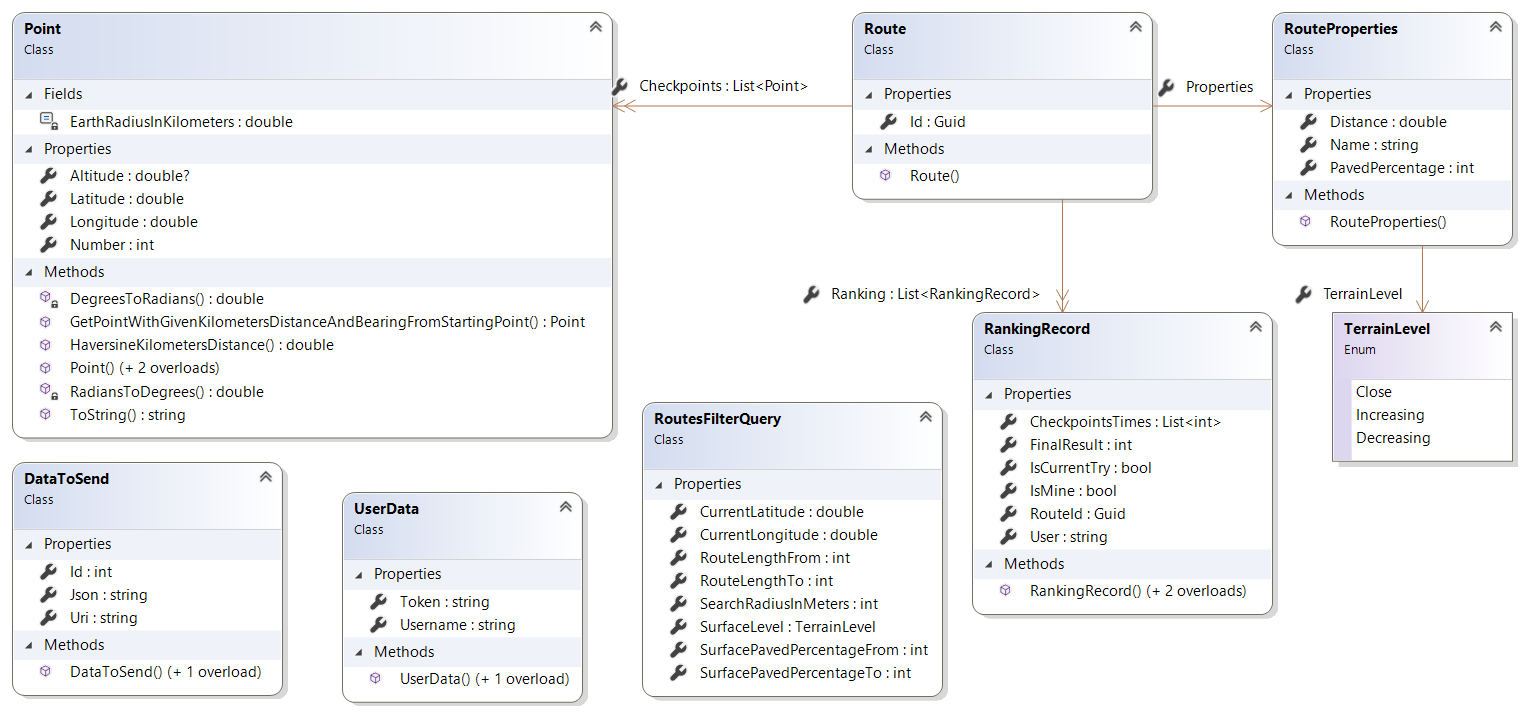
\includegraphics[width=\textwidth]{img/xamarin_model.png}
\caption{Diagram klas modelu danych aplikacji mobilnej [Opracowanie własne]}\label{image:xamarin_model}
\end{center}
\end{figure}
Ponad to model danych zawiera dwie dodatkowe klasy:
\begin{itemize}
\item{\textit{DataToSend}} - przechowuje dane w formacie JSON oraz adres URL. Pozwala podjąć ponowną, odłożoną w czasie próbę wysłania danych na serwer w przypadku gdy proces ten nie zakończy się sukcesem przy pierwszym podejściu.
\item{\textit{UserData}} - przechowuje dane o aktualnie zalogowanym użytkowniku: login użytkownika oraz token używany podczas komunikacji z serwerem.
\end{itemize}
\subsection{Aplikacja serwerowa}
Z racji podobieństwa do modelu danych zawartego w aplikacji mobilnej, który opisany został w rozdziale \ref{chap:model-mobilna}, w rozdziale niniejszym zostaną przybliżone jedynie nie omówione wcześniej aspekty. 

\begin{figure}[h]\label{fig:api_model}
\begin{center}
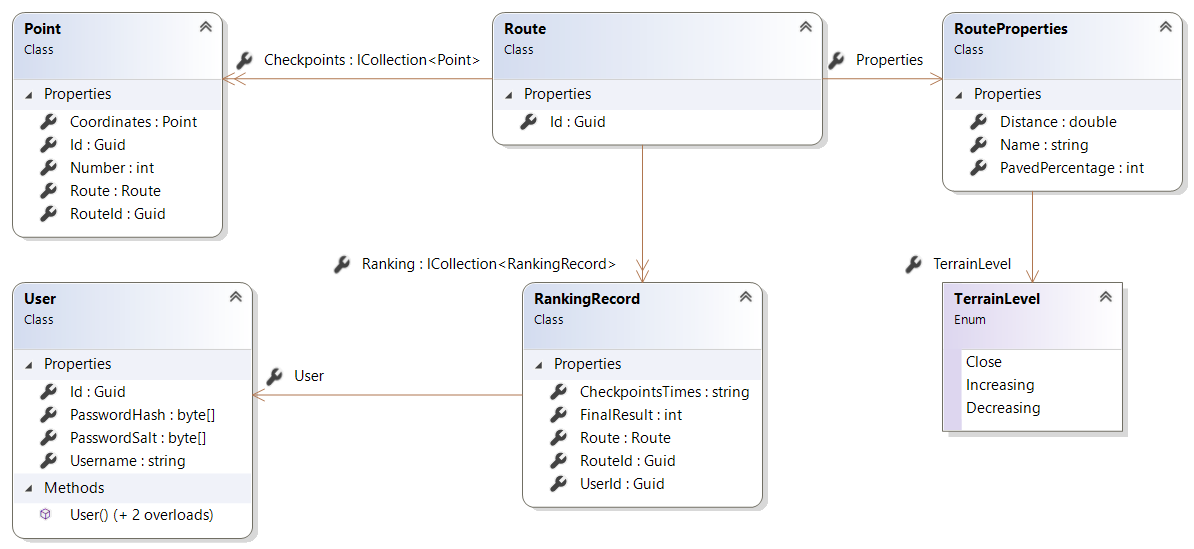
\includegraphics[width=\textwidth]{img/api_model.png}
\caption{Diagram klas modelu danych aplikacji serwerowej [Opracowanie własne]}\label{image:api_model}
\end{center}
\end{figure}

Jak widać na diagramie \ref{image:api_model} w modelu aplikacji serwerowej istnieje klasa \textit{User}. Reprezentuje ona konto użytkownika w systemie. Powiązanie tej klasy z klasą reprezentującą próbę na trasie, pozwala określić do którego z użytkowników należy konkretny wynik.

Współrzędne punktów trasy zapisywane przy użyciu typu danych \textit{Point}. Należy zaznaczyć, że nie jest to typ stworzony w ramach modelu danych, lecz należącą do przestrzeni nazw \textit{NetTopologySuite.Geometries}, występującą w środowisku .NET reprezentacją typu \textit{geography} istniejącego w systemie zarządzania bazą danych SQL Server. \textit{Geography} pozwala na przechowywanie współrzędnych geograficznych punktu (wraz z wysokością nad poziomem morza) w jednej kolumnie tabeli bazodanowej. \cite{geography-type}

\begin{figure}[h]
\begin{center}
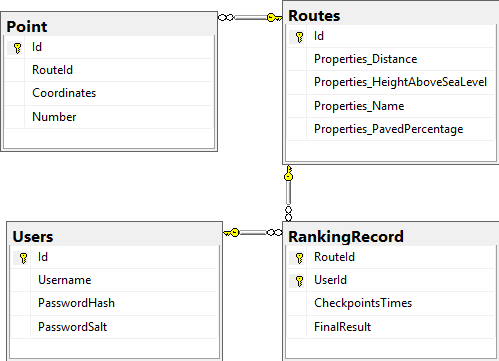
\includegraphics{img/er-diagram.png}
\caption{Diagram encji bazy danych [Opracowanie własne]}\label{image:db-structure}
\end{center}
\end{figure}

Zastosowanie mapowania obiektowo-relacyjnego pozwoliło na odwzorowanie modelu danych w formie bazy danych. Jej struktura została przedstawiona na rysunku \ref{image:db-structure}. Przed utworzeniem odpowiednich tabel konieczne było zdefiniowanie relacji pomiędzy polami tabel. Odpowiednią konfigurację umieszczono w klasie \textit{Context} znajdującej się w przestrzeni nazw \textit {Api.Entities} i przedstawiono na listingu \ref{listing:context}.

\begin{lstlisting}[caption={Konfiguracja mapowania relacyjno-obiektowego},label=listing:context]
protected override void OnModelCreating(
ModelBuilder modelBuilder)
{
    modelBuilder.Entity<Route>().HasMany(r => r.Checkpoints)
    	.WithOne(cp => cp.Route)
    	.HasForeignKey(cp => cp.RouteId);
    modelBuilder.Entity<Route>().OwnsOne(r => r.Properties);
    modelBuilder.Entity<Route>().HasMany(r => r.Ranking)
    	.WithOne(rr => rr.Route)
        .HasForeignKey(rr => rr.RouteId);

    modelBuilder.Entity<RankingRecord>().HasOne(rr => rr.User);
    modelBuilder.Entity<RankingRecord>()
    	.HasKey(rr => new { rr.RouteId, rr.UserId });

    base.OnModelCreating(modelBuilder);
}
\end{lstlisting}
Konfiguracja pozwoliła na utworzenie następujących relacji:
\begin{itemize}
\item{jeden do wielu pomiędzy tabelami reprezentującymi klasy \textit{Route}} oraz \textit{Point}
\item{jeden do wielu pomiędzy tabelami reprezentującymi klasy \textit{Route}} oraz \textit{RankingRecord}
\item{jeden do jednego pomiędzy tabelami reprezentującymi klasy \textit{RankingRecord} oraz \textit{User}}
\end{itemize}
Dzięki instrukcji z linii numer 7 dane z klas \textit{Route} oraz \textit{RouteProperties} zostały umieszczone w jednej tabeli. Pozwoliło to na uniknięcie łączenia tabel podczas pobierania danych. Typy wyliczeniowe nie wymagają osobnej tabeli i są przechowywane w postaci liczb, dlatego nie było potrzeby tworzenia dodatkowej struktury dla cechy \textit{poziom terenu}.

Warto zauważyć, że czasy osiągane na punktach kontrolnych są przechowywane jako łańcuch znaków (\textit{string}). Pozwoliło to uniknąć tworzenia dodatkowej tabeli i relacji jeden do wielu z tabelą reprezentującą klasę \textit{RankingRecord}. Mapowanie pomiędzy kolekcją a łańcuchem znaków odbywa się w klasie \textit{AutomapperConfig} znajdującej się w przestrzeni nazw \textit{Api.Mappers} i zostało przedstawione na listingu \ref{listing:collection-string-mapping}.
\begin{lstlisting}[caption={Mapowanie pomiedzy kolekcją a łańcuchem znaków},label=collection-string-mapping]
public static IMapper Initialize()
    => new MapperConfiguration(cfg =>
        {
         cfg.CreateMap<RankingRecord, RankingRecordDto>()
             .ForMember(dest => dest.CheckpointsTimes, opt =>
                    opt.MapFrom(src => src.CheckpointsTimes
                    .Split(" ", StringSplitOptions.None).Select(int.Parse)))
         cfg.CreateMap<RankingRecordDto, RankingRecord>()
             .ForMember(dest => dest.CheckpointsTimes,
                 opt => opt.MapFrom(src => 
                 string.Join(" ", src.CheckpointsTimes)))
        })
        .CreateMapper();
\end{lstlisting}

\section{Warstwa logiki biznesowej}
\subsection{Wyszukiwanie tras}
Wyszukiwanie tras odbywa się poprzez wysłanie zapytania z aplikacji mobilnej do aplikacji serwerowej. Ustalone przez użytkownika kryteria wyszukiwania są następnie przekazywane do bazy danych. Dzięki temu proces odfiltrowania tras ma miejsce tak wcześnie jak to możliwe i do aplikacji serwerowej, a następnie mobilnej trafiają tylko te trasy, które rzeczywiście spełniają ustalone kryteria. Diagram sekwencji tego procesu został pokazany na rysunku \ref{image:sekwencja_wyszukiwanie}. Kryteria wybrane przez użytkownika zapisane są w instancji klasy \textit{RoutesFilterQuery}, która pozwala zachować wszystkie informacje opisane w rozdziale \ref{chap:kryteria}. Obiekt ten jest przekazywany do części serwerowej systemu w celu dokonania odpowiedniej filtracji tras.

W momencie gdy zostanie wywołana metoda \textit{GetRoutesAsync} klasy \textit{RoutesRepository}, przekazany obiekt jest wykorzystany do określenia warunków, które muszą spełniać pobierane trasy. Działanie to zostało pokazane na listingu \ref{listing:filtracja_tras}. Warto podkreślić, że dzięki zastosowaniu typu \textit{geography} w tabeli bazy danych, możliwe jest policzenie odległości pomiędzy pozycją użytkownika a początkiem trasy bezpośrednio na poziomie bazy danych \cite{geography-type, geography-type2}. Warunek ten określa linia numer 8 listingu. Na podstawie określonych warunków generowane jest następnie zapytanie SQL wykonywane bezpośrednio na poziomie bazy danych.
\begin{lstlisting}[caption={Określenie warunków dla pobieranych tras},label=listing:filtracja_tras]
var routes = _context.Routes
	 .Where(r => r.Properties.PavedPercentage 
         >= query.SurfacePavedPercentageFrom
	&& r.Properties.PavedPercentage <= query.SurfacePavedPercentageTo)
        .Where(r => r.Properties.Distance >= query.RouteLengthFrom
        && r.Properties.Distance <= query.RouteLengthTo)
        .Where(r => r.Checkpoints.First(cp => cp.Number == 0)
        .Coordinates.IsWithinDistance(currentLocation,
        query.SearchRadiusInMeters));

if (query.SurfaceLevel > 0)
	routes = routes.Where(r => r.Properties.TerrainLevel 
	== (TerrainLevel)query.SurfaceLevel);
\end{lstlisting}
\begin{figure}[h]\label{fig:api_model}
\begin{center}
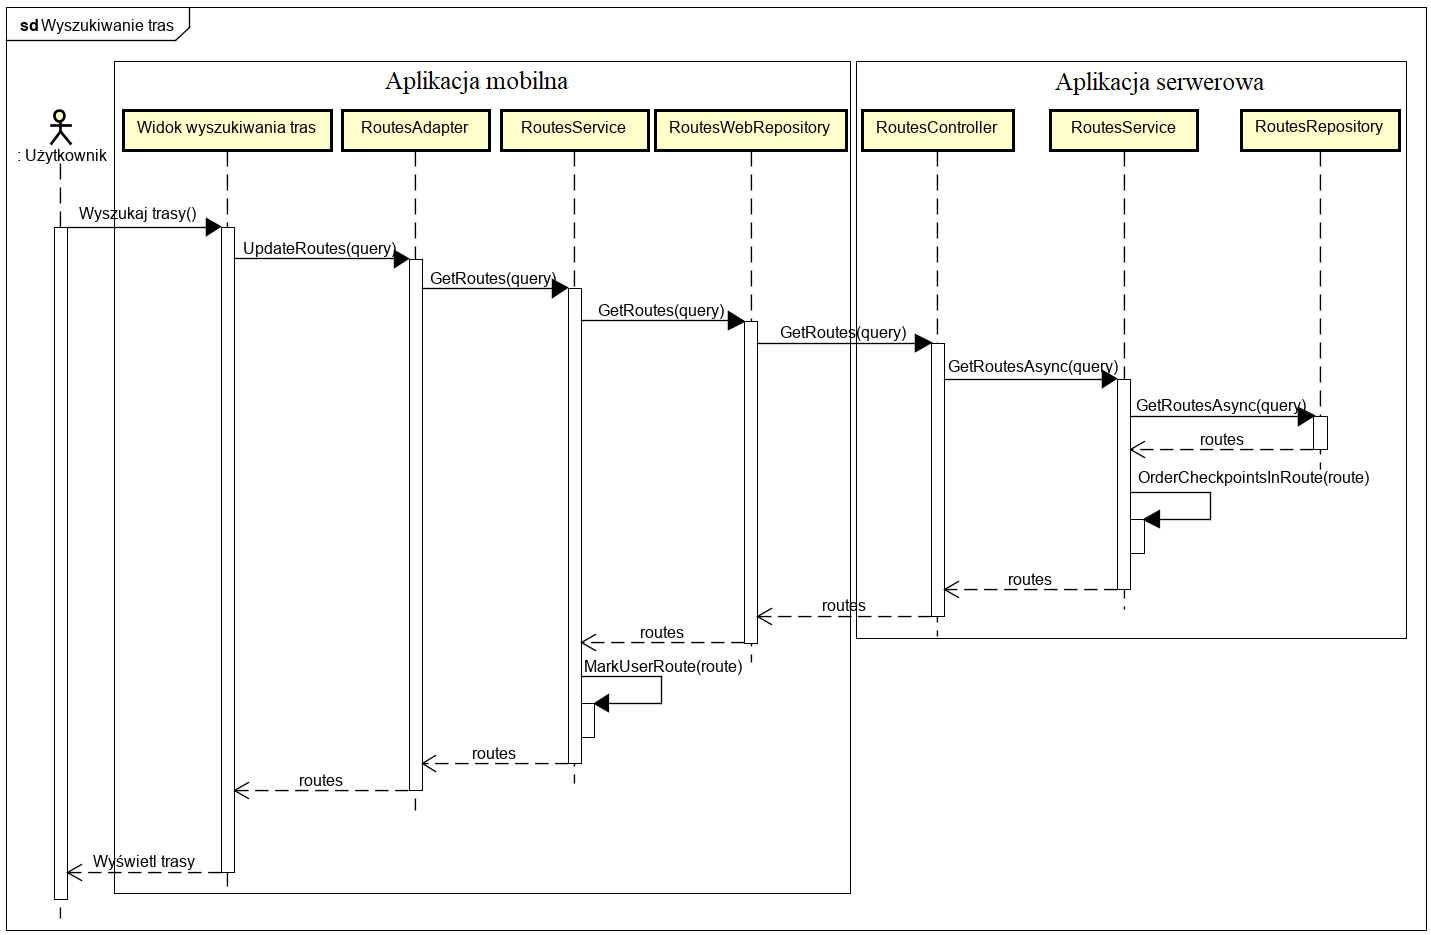
\includegraphics[width=\textwidth]{img/diagram_sekwencji_wyszukiwanie.png}
\caption{Diagram sekwencji procesu wyszukiwania tras [Opracowanie własne]}\label{image:sekwencja_wyszukiwanie}
\end{center}
\end{figure}
Po pobraniu danych z bazy danych, w klasie \textit{RoutesService} z przestrzeni nazw \textit{Api.Services} aplikacji serwerowej punkty kontrolne każdej trasy są sortowane według pola \textit{Number}, tak aby ich kolejność w kolekcji odpowiadała kolejności, którą powinny zajmować na trasie. Po przesłaniu danych o trasach z aplikacji serwerowej do aplikacji mobilnej, w klasie \textit{RoutesService} znajdującej się przestrzeni nazw \textit{Core.Services}, odbywa się aktualizacja własciwości \textit{IsMine}. Proces ten został pokazany na listingu \ref{listing:ismine}. Dzięki temu w interfejsie użytkownika możliwe jest wyróżnienie wyniku, który należy do biegacza.
\begin{lstlisting}[caption={Aktualizacja właściwości IsMine klasy Route},label=listing:ismine]
private void MarkUserRoute(Route route)
{
	var mineRankingRecord = route.Ranking
	.FirstOrDefault(r => r.User == _userData.Username);
	if (mineRankingRecord != null)
		mineRankingRecord.IsMine = true;
}
\end{lstlisting}

\subsection{Odbywanie treningu}
Implementacje treningu, który tworzy nową trasę jak i trening przeprowadzany w ramach istniejącej trasy, który zawiera w sobie dodatkowo element wirtualnej rywalizacji zawierają wspólną logikę, dlatego tak jak widać na rysunku \ref{image:trening-diagram}, skorzystano z mechanizmu dziedziczenia. Należy zwrócić uwagę, że klasy te zawierają kilka pól typu \textit{Action}. Dzięki nim możliwe jest aktualizowanie interfejsu użytkownika z poziomu metody klasy należącej do logiki biznesowej. W przypadku stworzenia aplikacji mobilnej przeznaczonej na inny system operacyjny, wystarczy przekazać odpowiednie implementacje metod odpowiedzialnych za aktualizację interfejsu użytkownika, a zostaną one wywołane. 

Metody \textit{Start} oraz \textit{Stop} służą do odpowiednio do rozpoczęcia i zakończenia treningu. Zawierają one logikę odpowiedzialną za dodanie obecnej próby użytkownika do rankingu oraz uruchomienie i zatrzymanie stopera. Dzięki stoperowi za każdym razem gdy upłynie jedna sekunda, aktualizowany jest interfejs użytkownika oraz wywoływana jest metoda \textit{ProcessUserLocation}, której implementacja zależna jest od typu treningu.
\begin{figure}[h]\label{fig:asdl}
\begin{center}
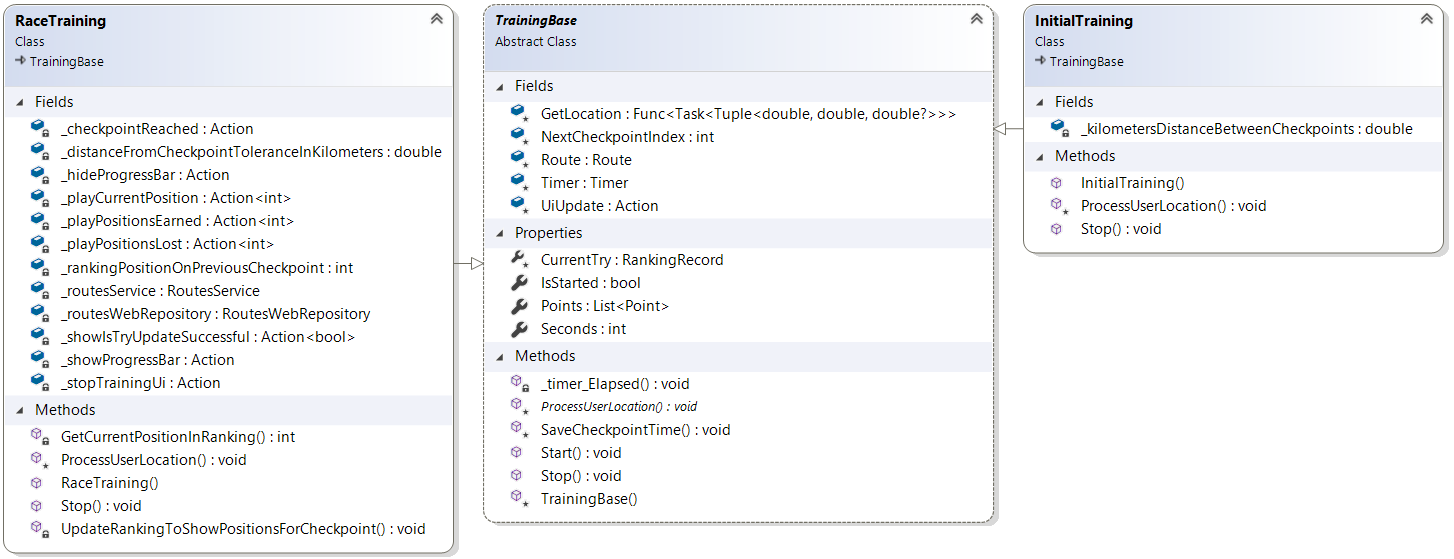
\includegraphics[width=\textwidth]{img/trening-diagram.png}
\caption{Diagram klas odpowiadających za przeprowadzanie treningów [Opracowanie własne]}\label{image:trening-diagram}
\end{center}
\end{figure}
\subsubsection{Trening tworzący trasę}
Za logikę obsługującą trening na nowej trasie odpowiada klasa \textit{InitialTraining}. Za każdym razem gdy wywołana zostanie metoda \textit{ProcessUserLocation}, podejmowana jest próba dodania do tworzonej trasy nowego punktu kontrolnego na podstawie obecnej pozycji biegacza. Aby punkt mógł zostać dodany, użytkownik musi znajdować się w pozycji nie mniejszej niż 10 metrów od ostatnio utworzonego punktu kontrolnego. Prawdziwość tego warunku jest sprawdzana w linii numer 6, 7 i 8 na listingu \ref{listing:add-point-initial}. Działanie ma to na celu uniknięcie problemu opisanego w rozdziale \ref{chap:wahania-pozycji}, którego wystąpienie spowodowałoby utworzenie skupiska punktów kontrolnych oddalonych od siebie o kilka metrów. Wyznaczenie odległości pomiędzy aktualną pozycją użytkownika, a ostatnio utworzonym punktem kontrolnym obliczana jest za pomocą formuły Haversine przytoczonej w rozdziale \ref{chap:haversine}. Jej implementacja została pokazana na listingu \ref{listing:haversine}. Współrzędne odczytywane są w stopniach, dlatego przed obliczeniem odległości, konieczne było wyznaczenie ich wartości w radianach.
\begin{lstlisting}[caption={Wyznaczenie odległości pomiędzy dwoma punktami},label=listing:haversine]
public static double HaversineKilometersDistance(Point point1,
	Point point2)
{
  var latitudeDelta = DegreesToRadians(point1.Latitude - point2.Latitude);
  var longitudeDelta = DegreesToRadians(
  	point1.Longitude - point2.Longitude);

  var firstPointLatitudeCos = Math.Cos(DegreesToRadians(point1.Latitude));
  var secondPointLatitudeCos = Math.Cos(
  	DegreesToRadians(point2.Latitude));

  var a = Math.Pow(Math.Sin(latitudeDelta / 2), 2)
  	+ firstPointLatitudeCos *
	secondPointLatitudeCos * Math.Pow(Math.Sin(longitudeDelta / 2), 2);
  var c = 2 * Math.Atan2(Math.Sqrt(a), Math.Sqrt(1 - a));
  var d = EarthRadiusInKilometers * c;

  return d;
}
\end{lstlisting}

\begin{lstlisting}[caption={Tworzenie punktów kontrolnych},label=listing:add-point-initial]
protected override async void ProcessUserLocation()
{
    var location = await GetLocation();
    var currentPosition = new Point(
    	location.Item1, location.Item2,location.Item3,NextCheckpointIndex);
    var distanceFromLastPoint = Route.Checkpoints.Any()
        ? Point.HaversineKilometersDistance(Route.Checkpoints.Last(),
        currentPosition)
        : _kilometersDistanceBetweenCheckpoints;
    if (distanceFromLastPoint >= _kilometersDistanceBetweenCheckpoints)
    {
        NextCheckpointIndex++;
        Route.Checkpoints.Add(currentPosition);
        SaveCheckpointTime();
    }
}
\end{lstlisting}
Wraz z utworzeniem punktu kontrolnego, zapisywany jest także czas, który upłynął od rozpoczęcia treningu. Oznacza to, że biegacz tworzący trasę, zostaje jednocześnie pierwszym użytkownikiem dodanym do rankingu.

W momencie gdy użytkownik postanawia zakończyć trening, wywołana zostaje metoda \textit{Stop}. Oprócz bazowej implementacji tej metody, zostaje także wykonany kod odpowiedzialny za utworzenie ostatniego punktu kontrolnego. Jest on tworzony niezależnie od odległości do przedostatniego punktu kontrolnego, a jego pozycja odpowiada pozycji użytkownika z momentu zakończenia treningu.

\subsubsection{Trening na zapisanej trasie oraz wirtualna rywalizacja}
Proces wirtualnej rywalizacji odbywa się wraz z rozpoczęciem treningu na stworzonej wcześniej trasie. Za obsługę obu tych elementów odpowiada klasa \textit{RaceTraining}. Metoda \textit{ProcessUserLocation} służy do zapisywania czasów, które biegacz osiągnął na każdym z punktów kontrolnych. Jej kod źródłowy został przedstawiony na listingu \ref{listing:add-point-race}.
\begin{lstlisting}[caption={Proces wirtualnej rywalizacji},label=listing:add-point-race]
protected override async void ProcessUserLocation()
{
  var location = await GetLocation();
  var currentLocation = (new Point(location.Item1,
    location.Item2, Seconds));
  var distance = Point.HaversineKilometersDistance(currentLocation,
    Route.Checkpoints[NextCheckpointIndex]);

  if (distance < _distanceFromCheckpointToleranceInKilometers)
  {
      NextCheckpointIndex++;

      SaveCheckpointTime();
      if (NextCheckpointIndex == Route.Checkpoints.Count)
      {
        Stop();
        _routesService.ProcessCurrentTry(Route, CurrentTry);

        _stopTrainingUi.Invoke();

        _showProgressBar.Invoke();
        var isSuccessful = await _routesWebRepository
		.CreateRankingRecordAsync(CurrentTry, Route.Id);
        _hideProgressBar.Invoke();
        _showIsTryUpdateSuccessful.Invoke(isSuccessful);
      }
      else
      {
        UpdateRankingToShowPositionsForCheckpoint(NextCheckpointIndex - 1);

        var currentPosition = GetCurrentPositionInRanking();
        if (currentPosition == 
          rankingPositionOnPreviousCheckpoint
            || _rankingPositionOnPreviousCheckpoint == 0)
        {
            _playCurrentPosition.Invoke(currentPosition);
        }
        else
        {
            if (currentPosition < _rankingPositionOnPreviousCheckpoint)
                _playPositionsEarned(
                _rankingPositionOnPreviousCheckpoint
                  - currentPosition);
            else
                _playPositionsLost(currentPosition
                  - _rankingPositionOnPreviousCheckpoint);
         }

        _rankingPositionOnPreviousCheckpoint = currentPosition;

        _checkpointReached.Invoke();
      }
  }
}
\end{lstlisting}
Biegacz musi znajdować się w odległości nie większej niż 10 metrów od następnego w kolejności punktu kontrolnego. Gdy ten warunek zostanie spełniony, bieżący czas od rozpoczęcia treningu zostaje zapisany. Odległość pomiędzy użytkownikiem a punktem kontrolnym wyznaczana jest za pomocą formuły haversine, której implementacja znajduje się na listingu \ref{listing:haversine}. Za każdym razem gdy punkt kontrolny zostanie osiągnięty, aktualizowany jest ranking. Odbywa się to poprzez posortowanie kolekcji \textit{Ranking} znajdującej się w instancji klasy \textit{Route} względem wartości, która reprezentuje czas osiągnięty przez wszystkich użytkowników na punkcie kontrolnym. Oprócz faktu, że pozycje w rankingu wyświetlonym na ekranie urządzenia zmieniają się wraz z trwaniem biegu, odtwarzane są komunikaty głosowe. Logika odpowiadająca za ten proces znajduje się w liniach 32-47 listingu \ref{listing:add-point-race} i jest implementacją warunków opisanych w rozdziale \ref{chap:zasada-tts}.

W momencie gdy zostaną osiągnięte wszystkie punkty kontrolne, trening jest automatycznie zakańczany, a próba użytkownika jest poddawana przetworzeniu. Scenariusz ten realizują linie 15-26 listingu \ref{listing:add-point-race}. Proces przetworzenia próby jest implementacją warunków opisanych w rozdziale \ref{chapter:sposob-rywalizacji} i został przedstawiony na listingu \ref{listing:przetworzenie-proby}.
\begin{lstlisting}[caption={Przetworzenie próby użytkownika},label=listing:przetworzenie-proby]
public void ProcessCurrentTry(Route route, RankingRecord currentTry)
{
    var lastTry = route.Ranking.SingleOrDefault(rr => rr.IsMine);
    if (lastTry == null) 
        return;
    if (currentTry.FinalResult < lastTry.FinalResult)
    {
        currentTry.IsMine = true;
        currentTry.IsCurrentTry = false;
        currentTry.User = lastTry.User;

        route.Ranking.Remove(lastTry);
    }
    else
        route.Ranking.Remove(currentTry);
}
\end{lstlisting}
Logika ta jest wykonywana na urządzeniu mobilnym, dzięki czemu użytkownik ma możliwość sprawdzenia końcowego rankingu wirtualnej rywalizacji. Warto zaznaczyć, że próba jest także wysyłana do aplikacji serwerowej, gdzie przetwarzana jest w ten sam sposób. Ma to miejsce nawet w przypadku, gdy końcowa lokata użytkownika w rankingu na urządzeniu mobilnym nie zmieniła się. Jest to spowodowane brakiem gwarancji, że ranking zapisany w bazie danych, jest nadal w tym samym stanie, co w momencie pobrania go na urządzenie mobilne przed rozpoczęciem treningu.

\subsection{Automatyczne przypisywanie cech do trasy}
Logikę odpowiedzialną za automatyczne przypisywanie cech umieszczono w klasie \textit{RoutesService}, która znajduje się w przestrzeni nazw \textit{Core.Services}. Została zaimplementowana zgodnie z opisem zawartym w rozdziale \ref{chap:przypisanie-cech}.
\subsubsection{Długość trasy}
Wyznaczenie długości polega na zsumowaniu odległości pomiędzy wszystkimi punktami trasy przy pomocy formuły haversine, której implementację pokazano na listingu \ref{listing:haversine}.
\begin{lstlisting}[caption={Wyznaczenie długości trasy},label=listing:dlugosc-trasy]
public void CalculateRouteDistance(Route route)
{
    var totalDistance = 0d;
    for (int i = 0; i < route.Checkpoints.Count - 1; i++)
    {
        totalDistance += Point.HaversineKilometersDistance(
        	route.Checkpoints[i], route.Checkpoints[i + 1]);
    }
    route.Properties.Distance = Math.Round(totalDistance, 2);
}
\end{lstlisting}
\subsubsection{Poziom terenu}
Wyznaczenie poziomu terenu zostało pokazane na listingu \ref{listing:poziom-terenu}. Wartość zmiennej \textit{terrainLevelDifferenceThresholdInPercentage} wyraża maksymalną procentową różnicę pomiędzy wysokością początkową a końcową dla której poziom terenu będzie uznany jako wyrównany. W tym przypadku wynosi ona 10\%.

Ponadto poziom terenu zostanie wyznaczony jako „wyrównany”, gdy nie udało się wyznaczyć wysokości któregokolwiek z punktów.
\begin{lstlisting}[caption={Wyznaczenie poziomu terenu},label=listing:poziom-terenu]
private void ResolveTerrainLevel(Route route)
{
    const int terrainLevelDifferenceThresholdInPercentage = 10;
    const double terrainLevelDifferenceThreshold =
    	1.0 * terrainLevelDifferenceThresholdInPercentage / 100 + 1;
    var startAltitude = route.Checkpoints.First().Altitude;
    var finishAltitude = route.Checkpoints.Last().Altitude;

    route.Properties.TerrainLevel = TerrainLevel.Close;
    if (startAltitude != null && finishAltitude != null)
    {
        if (startAltitude 
        	> finishAltitude * terrainLevelDifferenceThreshold)
        {
            route.Properties.TerrainLevel = TerrainLevel.Decreasing;
        }
        else if (finishAltitude 
        	> startAltitude * terrainLevelDifferenceThreshold)
        {
            route.Properties.TerrainLevel = TerrainLevel.Increasing;
        }
    }
}
\end{lstlisting}
\subsubsection{Twardość nawierzchni}
Za wyznaczenie tej cechy odpowiada klasa \textit{OsmService}. Główna metoda odpowiedzialna za to działanie została przedstawiona na listingu \ref{listing:twardosc-nawierzchni}. Metoda wywoływana w linii numer 3 listingu zajmuje się zbudowaniem odpowiedniego zapytania zgodnie z zasadami opisanymi w \cite{overpass-wiki}, wysłaniem go do serwisu OpenStreetMap \cite{osm} oraz zwróceniem otrzymanej odpowiedzi. W efekcie do zmiennej \textit{tags} zostają przypisane rodzaje nawierzchni dla każdego punktu trasy, natomiast zmienne \textit{PavedSurfaces} oraz \textit{UnpavedSurfaces} zawierają wszystkie możliwe utwardzone oraz nieutwardzone rodzaje nawierzchni zgodnie z tabelą \ref{table:rodzaje-nawierzchni} z rozdziału \ref{chapter:wyznaczenie-twardosc}. Na tej podstawie w liniach 4-7 wyznaczana jest procentowa twardość nawierzchni utworzonej trasy. 
W przypadku gdy nie uda się ustalić twardość nawierzchni (na przykład gdy z zewnętrznego serwisu nie uda się otrzymać żadnych informacji) twardość trasy zostaje ustalona jako wartość zmiennej \textit{DefaultSurfacePavement} wynosząca 50\%.
\begin{lstlisting}[caption={Wyznaczenie poziomu terenu},label=listing:twardosc-nawierzchni]
public async Task<int> ResolveRouteSurfaceTypeAsync(Route route)
{
  var tags = (await GetSurfaceTypesAsync(route.Checkpoints)).ToList();
  int pavedCount = tags.Count(t => PavedSurfaces.Contains(t));
  int unpavedCount = tags.Count(t => UnpavedSurfaces.Contains(t));

  var pavedPercent = 1.0 * pavedCount / (pavedCount + unpavedCount) * 100;
  if (double.IsNaN(pavedPercent))
      return DefaultSurfacePavement;

  return (int)Math.Round(pavedPercent);
}
\end{lstlisting}

\subsection{Brak połączenia z serwerem po zakończonym treningu}
Może zdarzyć się, że nie uda się zapisać treningu użytkownika, ponieważ urządzenie nie miało dostępu do internetu lub nastąpiła awaria serwera. W takim wypadku użytkownik utraciłby swoją próbę. Aby tego uniknąć, w momencie gdy nie uda się nawiązać połączenia z serwerem, dane o treningu w formacie JSON oraz adres pod który miały być wysłane zapisywane są w lokalnej bazie danych urządzenia. Następnie możliwe jest podjęcie ponownej próby wysłania zaległych danych. Proces ten został przedstawiony na listingu \ref{listing:overdue-data}. Metoda \textit{ProcessOverdueData} wywoływana jest przy każdym uruchomieniu aplikacji. Z lokalnej bazy danych pobierane są wszystkie zaległe treningi, a następnie po raz kolejny wysłane do części serwerowej aplikacji w metodzie wywoływanej w linii numer 6 listingu. W przypadku powodzenia tej operacji trening jest usuwany z lokalnej bazy danych.
\begin{lstlisting}[caption={Wyznaczenie poziomu terenu},label=listing:overdue-data]
public async Task ProcessOverdueData()
{
    var dataToSend = _userLocalRepository.GetDataToSend();
    foreach (var data in dataToSend)
    {
        var result = await _routesWebRepository
        	.SendJsonData(data.Json, data.Uri);

        if (result)
            _userLocalRepository.DeleteDataToSend(data.Id);
    }
}
\end{lstlisting}

\section{Warstwa interfejsu użytkownika}
\subsection{Internacjonalizacja}